\documentclass[slovak, 12pt, Times New Roman]{article}
\usepackage[slovak]{babel}
\usepackage[utf8]{inputenc} 
\usepackage[top=1in, bottom=1in, left=0.7in, right=0.7in]{geometry}
\usepackage{graphicx}
\usepackage{hyperref}
\hypersetup{
    colorlinks=true, %set true if you want colored links
    linktoc=all,     %set to all if you want both sections and subsections linked
    linkcolor=black,  %choose some color if you want links to stand out
}
\usepackage{fancyhdr}
\begin{document}
	\thispagestyle{fancy}
	\chead{Slovenská technická univerzita v Bratislave, Fakulta elektrotechniky a informatiky, Ilkovičova 3, 812 19 Bratislava}
	\topskip70mm
		\begin{center}\huge{Riaditel väznice\\\par}Semestrálna práca z DBS\end{center}
	\title{Softvérová špecifikácia WebRočenka}
	\date{}

	\begin{minipage}[b]{\textwidth}
	    \vspace{110mm}	 
	    \large   	\hspace{110mm} Vypracovali:\\
	    V Bratislave \hspace{82mm} Gabriel Kerekeš \\
	    1. Decembra 2014 \hspace{70mm} Jakub Jahnič \\
	    \vspace{-20mm} 
	\end{minipage}
	\topskip0pt

	\clearpage
	\tableofcontents
	\clearpage

	\section{Úvod}
		\subsection{Účel dokumentu}
			
		\subsection{Prehľad dokumentu}
	\section{Úloha}
		Kód úlohy: \textbf{D07} \\
		Názov úlohy: \textbf{Riaditeľ väznice} \\

		Bol Ste vymenovaný za riaditeľa menšej väznice, ktorá má A väzňov ubytovaných v B celách a máte k dispozícii C dozorcov (doplňte za A, B
		,C vhodné čísla). Vytvorte databázový systém, tak by Vaša väznica mohla efektívne fungovať. Potrebujete evidovať v databázovom systéme 
		väzňov s ich trestami a dátumom prepustenia, ich umiestnenie na celách, služby dozorcov, atď. Musíte mať prehľad o tom kedy bude ktorý 
		väzeň prepustený, sledovať jeho správanie a podľa tohto správania mu znížit, alebo zvýšiť trest. Podľa Vášho uváženia sledujte aj 
		ďalšie údaje napr. návštevy u väzňov, prijaté listy a balíčky, počet odpracovaných hodín dozorcov (prípadne aj väzňov), celkové 
		prehľady, atď.
	\section{Kocneptuálna úroveň}
		\subsection{Entity}
			Entity sme vyberali na základe toho aké údaje budeme potrebovať ukladať. Začali sme s entitami \textbf{VÄZEŇ}, \textbf{DOZORCA}, \textbf{CELA}.\\ Entita \textbf{VÄZEŇ} slúži na uchovávanie informácií o väzňoch, \textbf{DOZORCA} na uchovávanie údajov o dozorcoch a \textbf{CELA} informácie o celách. Pri navrhovaní entity \textbf{VÄZEŇ} sme boli donutení vytvoriť ďaľšie entity súvisiace s väzňami. Sú to \textbf{PRÁCA}, \textbf{ZÁVAŽNOSŤ TRESTU}, \textbf{PRIESTUPOK}, \textbf{POŠTA}. \textbf{PRÁCA} je entita, ktorá má v sebe uložené všetky práce, ktoré väzni môžu vykonávať. \textbf{ZÁVAŽNOSŤ TRESTU} má v sebe uložené závažnosti trestov aj s ichpopisom. \textbf{PRIESTUPOK} ukladá informácie o priestupkoch vykonaných väzňami. \textbf{POŠTA} ukladá informácie o pošte, ktorý väzni prijali alebo odoslali. Rovnako k entite \textbf{DOZORCA} sme museli vytvoriť entity \textbf{HODNOSŤ}, \textbf{BLOK}, \textbf{SLUŽBA}. \textbf{HODNOSŤ} je tabuľka uchovávajúca všetky hodnosti, ktoré môže dozorca dosiahnuť. Dozorca pracuje v určitom čase iba v jednom bloku. Všetky bloky väznice musia byť niekde uložené. Preto sme vytvorili entitu \textbf{BLOK}, aby sme vedeli určit v akom bloku dozorca pracujem, alebo v akom bloku sa nachádza cela. Entita \textbf{SLUŽBA} ukladá všetky služby, ktoré dozorca mal, alebo ešte len bude mať. Na určenie o akú službu sa jedná sme vytvorili entitut \textbf{TYP$\_$SLUŽBY} aby sa typ služby určoval jednoduchšie.
		\subsection{Atribúty}
			Atribúty sú vlastnosti entít. Zvolili sme ich následovne po diskusii so zákazníkom: \\
			\textbf{VÄZEŇ} - id, meno, priezvisko, cela, datum prijatia, datum prepustenia, priestupok, \\ závažnosť trestu, práca\\
			\textbf{ZÁVAŽNOSŤ TRESTU} - id, nazov\\
			\textbf{PRIESTUPOK} - id, id väzňa, dátum, popis\\
			\textbf{PRÁCA} - id, názov, odmena\\
			\textbf{POŠTA} - id, id väzňa, cinnost\\
			\textbf{DOZORCA} - id, meno, priezvisko, blok, hodnosť, plat \\
			\textbf{HODNOSŤ} - id, nazov, platová skupina\\
			\textbf{PLATOVÁ SKUPINA} - id, minimálny plat, maximálny plat\\
			\textbf{BLOK} - id, názov bloku, počet ciel, kapacita, obsadenosť, úroveň stráženia\\
			\textbf{CELA} - id, kapacita, obsadenosť\\
			\textbf{SLUŽBA} - id, id dozorcu, id typu sluzby\\
			\textbf{TYP SLUŽBY} - id, nazov sluzby, cas od, cas do\\
		\subsection{Matrix diagram}
			\begin{figure}[!htb]
				\centering
				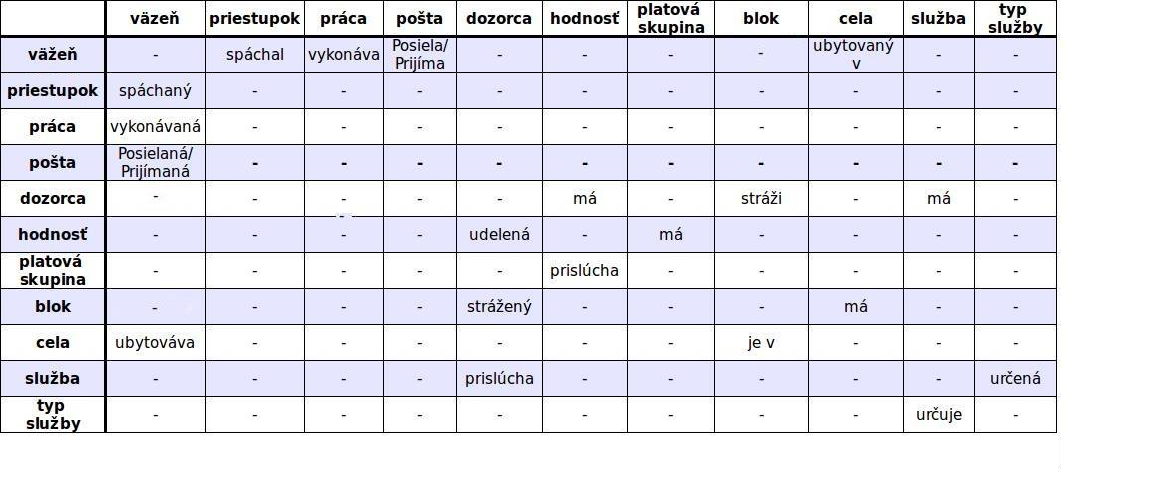
\includegraphics[scale=0.45]{matrixDia.png}
				\caption{Matrix diagram}
				\label{fig:Reinforcement}
			\end{figure}
		\subsection{Vzťahy medzi entitami}
			\textbf{Väzeň - Práca} \\
				Kardinalita: N:1 Jednu prácu môže vykonávať viac väzňov, avšak väzeň môže vykonávať iba jednu prácu v daný čas.\\
				Parcialita: Väzeň nemusí vykonávať žiadnu prácu, avšak práca musí byť vykonávaná nejakým väzňom.\\ 
				Transferabilita: Väzňovi môže byť práca hocikedy zmenená a takisto aj práca môže byť vykonávaná inými väzňami.\\ \\
			\textbf{Väzeň - Závažnosť trestu} \\
				Kardinalita: N:1 Jeden typ závažnosti trestu môže mať viac väzňov, avšak väzeň môže mať iba jeden typ závažnosti trestu. \\
				Parcialita: Väzeň musí mať nejaký typ závažnosti trestu, avšak závažnosť trestu nemusí prislúchať nejakému väzňovi.\\ 
				Transferabilita: Závažnosť trestu väzňa sa nemôže meniť.\\ \\
			\textbf{Väzeň - Priestupok} \\
				Kardinalita: 1:N Jeden priestupok bude zaznamenaný pre jedného väzňa, a jeden väzeň mohol spáchať viacej priestupkov.
				\\
				Parcialita: Väzeň nemusí spáchať priestupok, avšak priestupok musí mať svojho vinníka.\\ 
				Transferabilita: Po vykonaní priestupku sa už väzeň, ktorý ho vykonal meniť nemôže.\\ \\
			\textbf{Väzeň - Pošta} \\
				Kardinalita: 1:N Poštu môže odoslať/prijímať len jeden väzeň, avšak viac väzňov môže odoslať/prijímať poštu.\\
				Parcialita: Väzeň nemusí odosielať/prijímať pošty, avšak pošta musí mať svojho odosielateľa/prijímateľa.\\ 
				Transferabilita: Pošta, ktorá už bola odoslaná/prijatá svojho odosielateľa/príjemcu nezmení.\\ \\
			\textbf{Väzeň - Cela} \\
				Kardinalita: N:1 Cela môže ubytovávať viacerých väzňov, avšak väzeň môže byť ubytovaný len v jednej cele. \\
				Parcialita: Väzeň musí byť ubytovaný v cele, avšak cela nemusí ubytovávať žiadneho väzňa.\\ 
				Transferabilita: Väzeň môže byť presúvaný medzi celami.\\ \\
			\textbf{Dozorca - Hodnosť} \\
				Kardinalita: N:1 Jednu hodnosť môže mať viacero dozorcov, avšak jeden dozorca môže mať len jednu hodnosť.\\
				Parcialita: Dozorca musí mať hodnosť, a taktiež hodnosť musí prislúchať nejakému dozorcovi.\\ 
				Transferabilita: Dozorca môže byť povýšený.\\ \\
			\textbf{Dozorca - Blok} \\
				Kardinalita: N:1 Blok môže byť strážený viacerými dozorcami, avšak dozorca môže strážiť len jeden blok naraz.\\
				Parcialita: Dozorca musí strážiť nejaký blok, avšak blok nemusí byť strážený žiadnym dozorcom.\\ 
				Transferabilita: Dozorca môže byť preradený na iný blok.\\ \\
			\textbf{Dozorca - Služba} \\
				Kardinalita: 1:N Jedna služba môže prislúchať len jednému dozorcovi, avšak jeden dozorca môže mať viacero služieb.\\
				Parcialita: Dozorca musí byť prihlásený na službu a služba musí mať svojho vykonávateľa.\\ 
				Transferabilita: Už existujúca služba môže zmeniť svojho vykonávateľa (napr. keď dozorca ochorie)\\ \\
			\textbf{Hodnosť - Platová skupina} \\
				Kardinalita: N:1 Jedna platová skupina môže obsahovať viacero hodností, avšak jedna hodnosť môže byť len v jednej platovej 
				skupine.\\
				Parcialita: Hodnosť musí byť zapísaná v nejakej platovej skupine, a taktiež platová skupina musí obsahovať nejakú hodnosť.\\ 
				Transferabilita: Hodnosť bude vždy patriť do tej istej platovej skupiny. (platová skupina by sa mohla zmeniť iba pri väčších organizačných zmenách, ktoré zanedbáme).\\ \\
			\textbf{Blok - Cela} \\
				Kardinalita: 1:N Jedna cela môže byť len v jednom bloku, avšak jeden blok môže obsahovať viacero ciel.\\
				Parcialita: Blok musí obsahovať celu, a taktiež cela musí byť v nejakom bloku.\\ 
				Transferabilita: Cela blok len tak nezmení.\\ \\
			\textbf{Služba - Typ služby} \\
				Kardinalita: N:1 Jeden typ služby môže mať viacero služieb, avšak jedna služba môže byť len jedným typom služby.\\
				Parcialita: Služba musí byť nejakým typom služby, avšak typ služby nemusí mať žiadnu službu.\\ 
				Transferabilita: Služba typ služby nezmení, môžu sa vymeniť iba vykonávatelia služby.\\ \\
		\clearpage
		\subsection{ERA diagram}
			\begin{figure}[!htb]
				\centering
				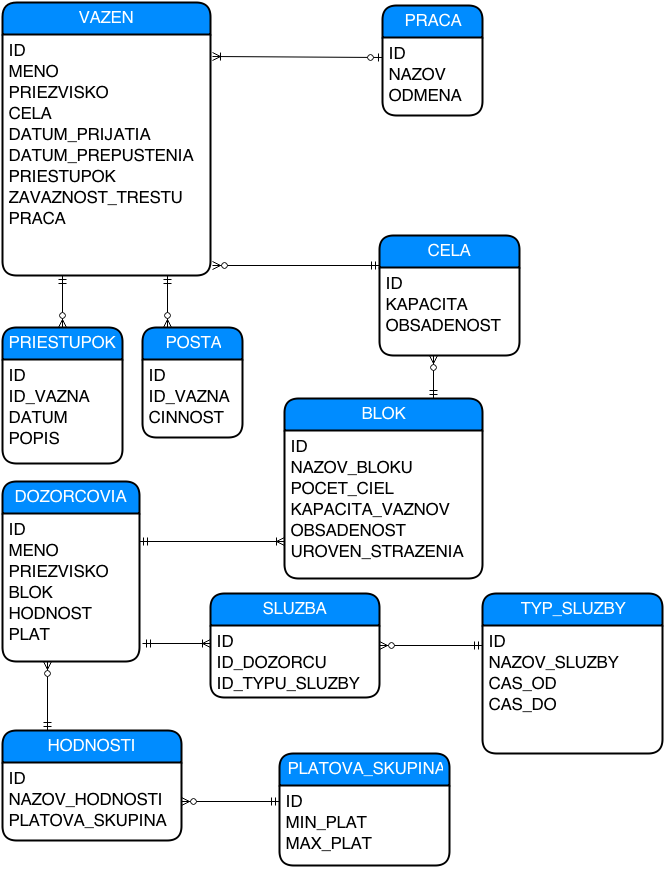
\includegraphics[scale=0.6]{ERAdia.png}
				\caption{ERA diagram}
				\label{fig:Reinforcement}
			\end{figure}
		\subsection{Prehľad požiadaviek používateľa databázového systému}
			Budeme potrebovať evidovať všetkých väzňov. Ich dátumy uväznenia, dátumy prepustenia, poštu, ktorú prijímajú/odosielajú, závažnosť 
			ich trestov, ich prácu vo väznici a priestupky, ktoré vykonali. Podľa ich priestupkov budeme vedieť určovať ich správanie a podľa 
			toho im zvyšovať/znižovať ich trest. \\
			Taktiež budeme potrebovať evidovať informácie o všetkých dozorcoch. Akú majú hodnosť, plat a aký blok strážia. Každá hodnosť má 
			pridelenú platovú skupinu do ktorej zapadá. O platovej skupine potrebujeme uchovávať len jej názov, maximálny a minimálny plat. 
			Dozorcovia tiež majú služby, ktoré tiež treba uchovávať. Služby sú rôzne, preto budeme potrebovať ukladať aj typy služieb. Typ 
			služby má byť určený nejakým názvom, časom začiatku služby a časom škončenia služby. Máme tri základné typy služieb a to rannú, 
			poobednú a nočnú, ale napríklad keď dozorca môže pracovať od 10:00 do 12:00, malo by toto byť vytvorené ako nový typ služby.	\\
			Naša väznica je rozdelená na bloky. V každom bloku je niekoľko ciel a v každej cele môže bývať viacero väzňov. Čiže systém by mal 
			mať uložené všetky naše cely, ich kapacitu a v akom bloku sa nachádzajú. Pri blokoch potrebujeme mať tiež uloženú ich kapacitu, ale 
			ešte aj ich úroveň stráženia znázornenú číslom. 
	\section{Logická úroveň}
		\subsection{Normalizácia}
			Všetky naše tabuľky sú navrhnuté podľa 1., 2. aj 3. normálovej formy. Aby bola splnená prvá normálová forma, musia byť všetky 
			atribúty entít atomické, čo znamená že napr. meno a priezvisko nebudú uchované v jednom stĺpci ale budú rozdelené do dvoch stĺpcov. 
			Pre druhú normálovú formu musí byť splnené, že každý atribút, ktorý nieje primárnym kľúčom je na ňom úplne závislý. ??? V tretej 
			normálovej forme je tabuľka vtedy, keď všetky jej atribúty, ktoré nie sú primárnym kľúčom, sú na sebe nezávislé. Ak by takýto atribút existoval, bolo by nutné ho presunúť do novej entity. Tretia normálova forma je dôvodom pre relatívne veľký počet entít.
		\subsection{Voľba a stanovenie identifikátorov, primárnych kľúčov, pre definované entity}
			Všetky naše entity majú ako primárny kľúč ID. Spravili sme tak z dôvodu zrozumitelnejšieho a na pamäť menej náročneho prepojenia dvoch entít.
		\clearpage
		\subsection{Relačná schéma}	
			\begin{figure}[!htb]
				\centering
				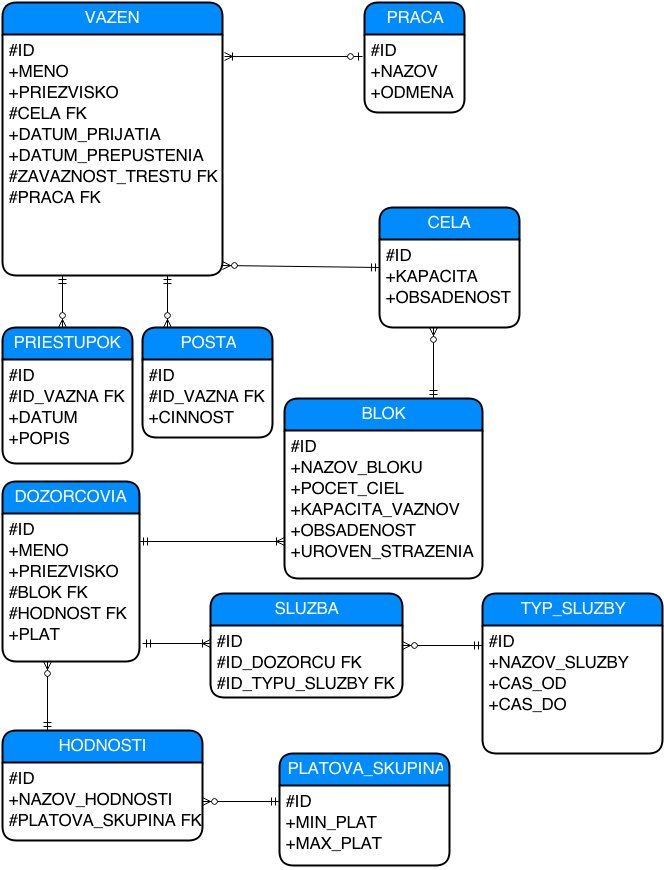
\includegraphics[scale=0.6]{relacnyDia.png}
				\caption{Relačný diagram}
				\label{fig:Reinforcement}
			\end{figure}
	\section{Implementačná úroveň}
		\subsection{Slovný popis návrhu}
			\subsubsection{Dátove typy}
				Mená sme zvolili ako dátový typ VARCHAR2 s rozsahom 12 a priezviská s rozsahom 18. Predpokladáme, že takýto rozsah nám bude stačiť, keďže pravdepodobne budeme pracovať so slovenskými menami.
				Pre názov práce, názov priestupku, názov hodnosti, názov služby a názov trestu sme použili dátový typ VARCHAR2 s rozsahom 12. 
				Pre úroveň stráženia a závažnosť trestu použijeme dátový typ NUMBER s rozsahom 1. Keďže úrovne stráženia a závažnosti sa značia od 1-9, tak nám takýto rozsah bude stačiť. 
				Pre plat, počet ciel, kapacitu väzňov v bloku, obsadenosť v bloku a pre pracovné odmeny sme zvolili dátový typ NUMBER s rozsahom 5. Takýto rozsah nám bude stačiť. 
				Pre každé ID sme zvolili dátový typ NUMBER s rozsahom 5 pre jasnejšiu identifikáciu a dostatočný priestor. 
				Dátumy sa ukladajú ako reťazce pohyblivej dĺžky s maximálnym rozsahom 10 - VARCHAR2(10).
				Čas od a čas po v typoch služieb ukladáme ako NUMBER(2,1), pretože sa tieto časy budú značiť ako napr. 6. alebo 6.5, či 12.5.
				Pre kapacitu väzňov a obsadenosti väzňov v celách nám stačí dátový typ NUMBER s rozsahom 1, pretože žiadna cela nebude môcť obsahovať viac ako 2 väzňov, a teda ani obsadenosť nebude vyššia. 
				Pre minimum platovej skupiny, maximum platovej skupiny a plat dozorcu budeme potrebovať dátový typ NUMBER(5,2), teda NUMBER s rozsahom 5 číslic a s presnoťou 2 desatinným miestach. Keďže plat môže byť aj napr. 540,55.
			\subsubsection{Určenie DEFAULT hodnôt pre stĺpce}
				Zadanie defaultnej hodnoty má zmysel pri vytváraní nového väzňa, kde za dátum uväznenia zadáme aktuálny dátum, získaný orezaním a zmenou typu systémového času. 
				Takisto aj dátum priestupku sa bude riešiť rovnakým spôsobom, a teda defaultnov hodnotou bude deň pripísania priestupku.
				Pre atribút práca, v entite väzeň, môžeme zadať defaultnú hodnotu NULL, pretože tento atribúť zmeníme, až keď mu dozorcovia pridelia prácu. 
				Pre obsadenosť bloku a obsadenosť ciel môžeme zadať defaultnú hodnotu NULL, pretože hneď po vytvorení v bloku nie je žiaden väzeň a takisto pri vytvorení cely nie je v cele žiaden väzeň. 
			\subsubsection{Obmedzenia}
				ja
		\subsection{Fyzický model}
		\subsection{Prehľad potrebných SQL dopytov}
			\subsubsection{Vkladanie údajov do tabuliek, zmena hodnôt stĺpcov}
				INSERT INTO VAZNI VALUES(10000,'Ferko','Mrkvcicka',default,'12/10/2022',10,default,default,5);\\
				INSERT INTO DOZORCOVA VALUES(50,'Rastislav','Dolina');\\
				INSERT INTO POSTY VALUES(11,12311,'poslal');\\
				INSERT INTO BLOKY VALUES(1432,'lave kridlo',122,244,default,3);\\
				INSERT INTO CELY VALUES(10002,2,default);\\
				INSERT INTO HODNOSTI VALUES('12','Plukovnik',1112);\\
				INSERT INTO PLATOVE$\_$SKUPINY VALUES(214,600,900);\\
				INSERT INTO PRACE VALUES(65,'pradelna',100);\\
				INSERT INTO SLUZBY VALUES(934,1235,592);\\
				INSERT INTO TYPY$\_$SLUZIEB VALUES(521,'ranna',6,14.5);\\
				INSERT INTO ZAVAZNOSTI$\_$TRESTOV VALUES(11,3);\\
				INSERT INTO PRIESTUPKY VALUES(9812,531,default,'bitka');\\
			\subsubsection{Vymazávanie údajov}
	\section{Záver}

\end{document}